\documentclass[11pt]{article}

\usepackage[margin=1in]{geometry}
\usepackage{setspace}
\usepackage{graphicx}
\usepackage{booktabs}
\usepackage[colorlinks=true, linkcolor=blue, urlcolor=blue]{hyperref}
\usepackage{float}
\usepackage{xcolor}
\usepackage{amsmath}
\usepackage{enumitem}

\graphicspath{{output/graphs/descriptives/}}

\title{Eureka: Decomposing AI Usage into Automation and Augmentation\\[6pt]
       \large A Verb-Based Approach Using Bloom's Taxonomy\\
       and the Anthropic Economic Index}
\author{Leyao Wang\\
        \small University of Virginia}
\date{April 2026 --- Working Notes}

\begin{document}
\maketitle
\thispagestyle{empty}

\begin{abstract}
\noindent
Existing measures of AI exposure (Eloundou et al.\ 2024; Felten et al.\ 2021) quantify \emph{whether} AI can perform occupational tasks, but not \emph{how} it is used --- as a substitute for human labor or a complement to it.  I propose a method to decompose AI usage into \textbf{automation} and \textbf{augmentation} channels using the semantic structure of task descriptions.  The key insight: the \emph{verb} in an O*NET task statement signals cognitive complexity.  Lower-order verbs (calculate, process, sort) describe tasks AI can execute independently; higher-order verbs (analyze, evaluate, design) describe tasks where AI assists human judgment.  Classifying verbs via Bloom's Taxonomy and weighting by revealed AI usage from the Anthropic Economic Index yields two independent, occupation-level indices.  Preliminary descriptive results show meaningful variation across occupations and occupation groups.
\end{abstract}

\clearpage
\onehalfspacing

%==================================================
\section{Motivation}
%==================================================

The recent literature on AI and labor markets relies on measures of AI \emph{exposure} --- scores that predict how much of an occupation's task bundle can be performed by large language models.  The leading measure, Eloundou et al.\ (2024), assigns each occupation a score based on GPT-4's assessment of whether it could reduce task completion time by 50\%.

These measures answer: \textbf{can AI do this task?}  They do not answer: \textbf{how do humans actually use AI for this task?}

This distinction matters.  A task that AI \emph{can} do may in practice be:
\begin{itemize}
  \item \textbf{Automated}: the human delegates the task entirely to AI (substitution).
  \item \textbf{Augmented}: the human uses AI as a tool while retaining judgment (complementarity).
\end{itemize}

The Anthropic Economic Index (Handa et al.\ 2025) provides the missing piece: revealed AI usage data from millions of Claude conversations, mapped to O*NET occupational tasks.  Their aggregate finding --- 57\% augmentation, 43\% automation --- confirms that both channels are empirically relevant.  However, they do not release the augmentation/automation classification at the task or occupation level.

\textbf{This note proposes a method to construct that decomposition.}

%==================================================
\section{The Idea: Verbs as Cognitive Signatures}
%==================================================

Every O*NET task statement follows the structure: \textbf{Verb} + object + context.

\begin{quote}
\small
``\textbf{Calculate} tax liabilities using financial records.'' \\
``\textbf{Evaluate} treatment options for patients with chronic conditions.'' \\
``\textbf{Design} database systems to store and retrieve information.''
\end{quote}

The verb carries information about the \emph{cognitive mode} of the task.  ``Calculate'' is execution --- deterministic, no judgment required.  ``Evaluate'' is judgment --- the human weighs evidence and decides.  ``Design'' is creation --- the human produces something new.

This maps directly onto \textbf{Bloom's Taxonomy} (1956; revised Anderson \& Krathwohl 2001), which classifies cognitive processes into six levels of increasing complexity:

\begin{center}
\begin{tabular}{clcl}
\toprule
Level & Category & & Mapping \\
\midrule
1 & Remember    & \multirow{3}{*}{\textcolor{red}{$\Rightarrow$ \textbf{Automation}}} & \multirow{3}{*}{\small Tasks AI can execute independently} \\
2 & Understand  & & \\
3 & Apply       & & \\
\midrule
4 & Analyze     & \multirow{3}{*}{\textcolor{blue}{$\Rightarrow$ \textbf{Augmentation}}} & \multirow{3}{*}{\small Tasks where AI assists human judgment} \\
5 & Evaluate    & & \\
6 & Create      & & \\
\bottomrule
\end{tabular}
\end{center}

The mapping is intuitive: lower-order cognitive tasks (remember, apply, execute) are precisely the tasks that AI can fully automate --- they require following procedures, not exercising judgment.  Higher-order tasks (analyze, evaluate, create) are where AI serves as a complement --- it provides information, drafts options, or generates candidates, but the human makes the final call.

%==================================================
\section{Construction}
%==================================================

\subsection{Data}

\begin{enumerate}
  \item \textbf{Anthropic Economic Index} --- \texttt{task\_penetration.csv}: 17,998 O*NET task statements, each with a \emph{penetration score} measuring the share of Claude conversations that involve that task.  Source: Handa et al.\ (2025), via HuggingFace.
  \item \textbf{O*NET Task-to-Occupation Crosswalk} --- \texttt{onet\_task\_statements.csv}: maps each task to its associated O*NET-SOC occupation code, with task type (Core/Supplemental) and incumbents responding.
\end{enumerate}

\subsection{Steps}

\begin{enumerate}
  \item \textbf{Extract the root verb} from each task statement using spaCy NLP parsing.
  \item \textbf{Classify the verb} into a Bloom's Taxonomy level (1--6) using a predefined dictionary of $\sim$300 verbs covering $\sim$95\% of tasks.
  \item \textbf{Score each task}:
  \begin{itemize}
    \item $\text{is\_auto} = 1$ if Bloom level $\in \{1, 2, 3\}$, else 0
    \item $\text{is\_aug} = 1$ if Bloom level $\in \{4, 5, 6\}$, else 0
  \end{itemize}
  \item \textbf{Aggregate to occupation level}:
  \begin{align}
    \text{AutomationIndex}_o &= \frac{\sum_{t \in T_o} \text{penetration}_t \times \text{is\_auto}_t \times w_t}{\sum_{t \in T_o} w_t} \\[6pt]
    \text{AugmentationIndex}_o &= \frac{\sum_{t \in T_o} \text{penetration}_t \times \text{is\_aug}_t \times w_t}{\sum_{t \in T_o} w_t}
  \end{align}
  where $w_t = (\text{Core} \times 2 + \text{Supplemental} \times 1) \times \text{Incumbents Responding}$.
\end{enumerate}

\textbf{Key property}: the two indices are \emph{independent}.  An occupation can score high on both (AI is heavily used for both execution and judgment tasks), low on both (AI barely touches it), or any combination.

\subsection{Why Not Embeddings?}

An earlier attempt used sentence-transformer embeddings + K-means clustering on full task statements.  This failed: O*NET task statements are written in a standardized bureaucratic style, so embeddings cluster by \emph{domain} (healthcare vs.\ finance) rather than by \emph{cognitive mode} (execute vs.\ analyze).  The Bloom's verb approach avoids this by extracting the cognitive-mode signal directly from the verb, which is orthogonal to the domain content of the task.

%==================================================
\section{Validation}
%==================================================

\begin{figure}[H]
\centering
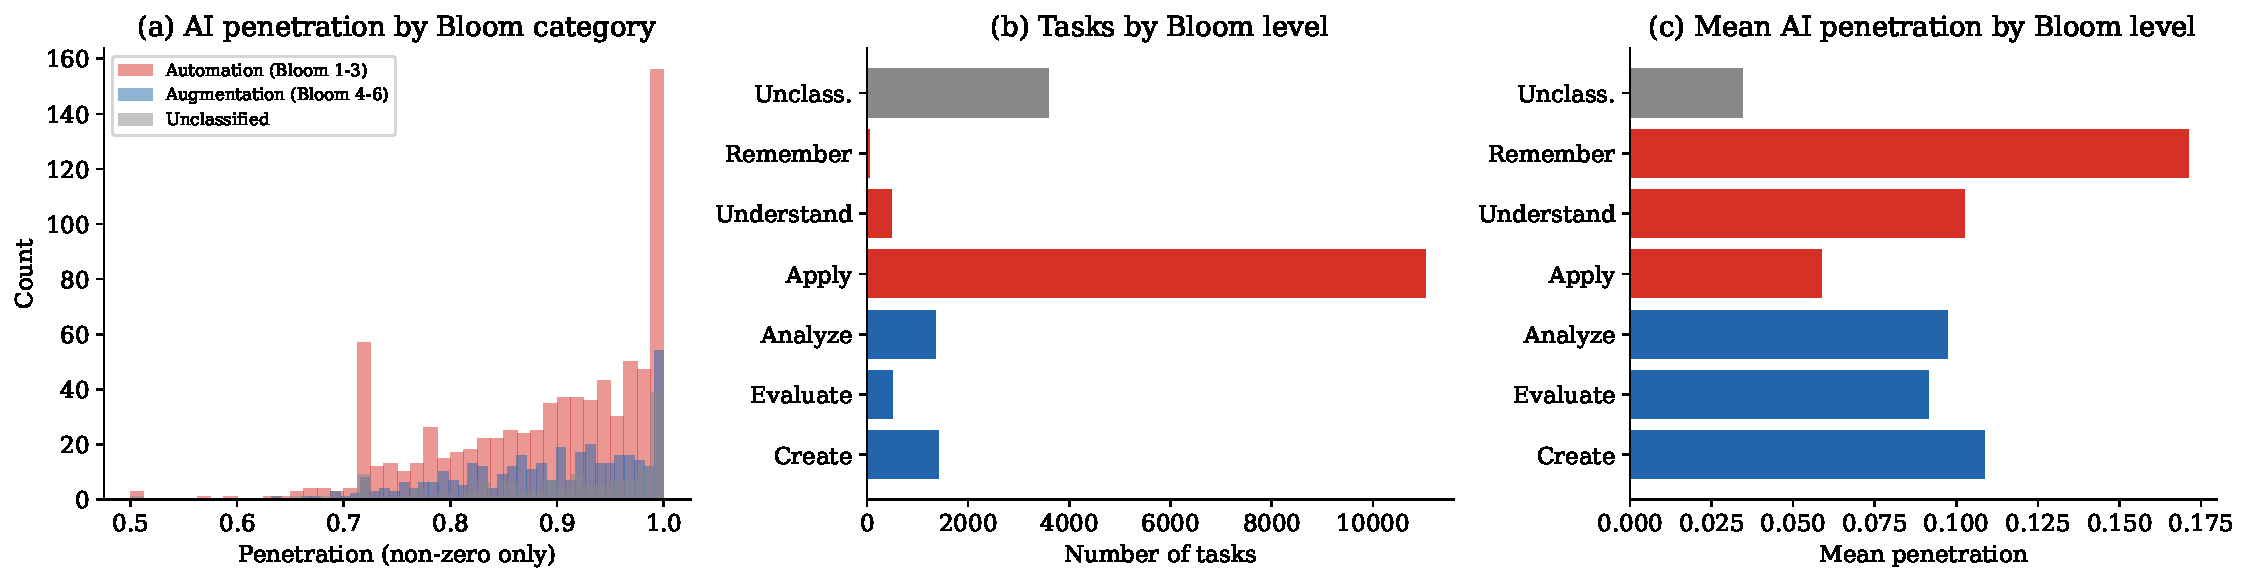
\includegraphics[width=\textwidth]{bloom_validation.pdf}
\caption{Bloom classification validation.  (a) Penetration distribution by category: both automation and augmentation tasks show non-trivial AI usage.  (b) Task count by Bloom level: ``Apply'' (level 3) dominates, reflecting O*NET's emphasis on procedural tasks.  (c) Mean penetration by Bloom level.}
\label{fig:bloom_validation}
\end{figure}

%==================================================
\section{Results: Occupation-Level Indices}
%==================================================

\begin{figure}[H]
\centering
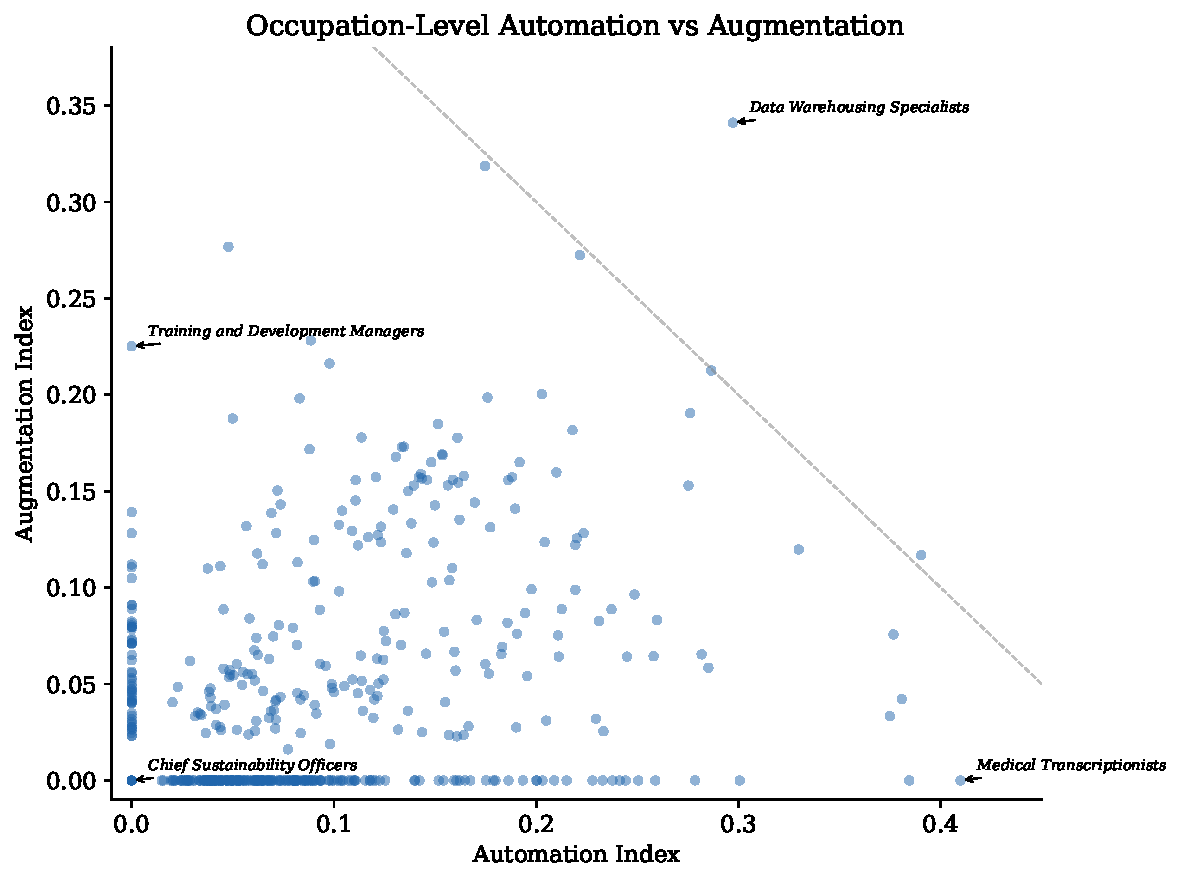
\includegraphics[width=0.85\textwidth]{auto_vs_aug_scatter.pdf}
\caption{Occupation-level automation vs.\ augmentation index (detailed O*NET-SOC occupations).  Each dot is one occupation.  Four corner representatives labeled.  The indices are independent: occupations span the full two-dimensional space.}
\label{fig:scatter}
\end{figure}

\begin{figure}[H]
\centering
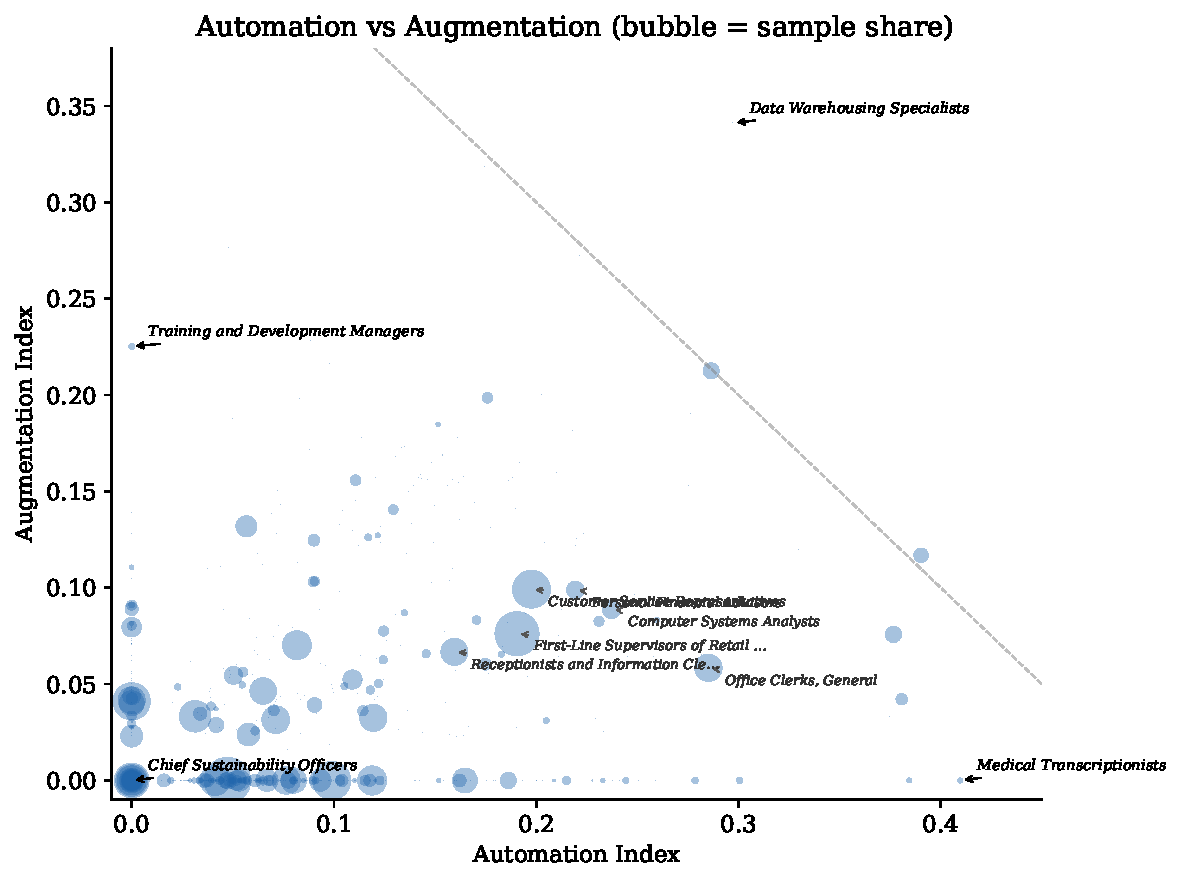
\includegraphics[width=0.85\textwidth]{auto_vs_aug_bubble.pdf}
\caption{Same as Figure~\ref{fig:scatter}, with bubble size proportional to each occupation's share of the CPS-ASEC sample.  Large bubbles in the interior represent common occupations (e.g.\ managers, accountants, teachers) that face both automation and augmentation pressure.}
\label{fig:bubble}
\end{figure}

\begin{figure}[H]
\centering
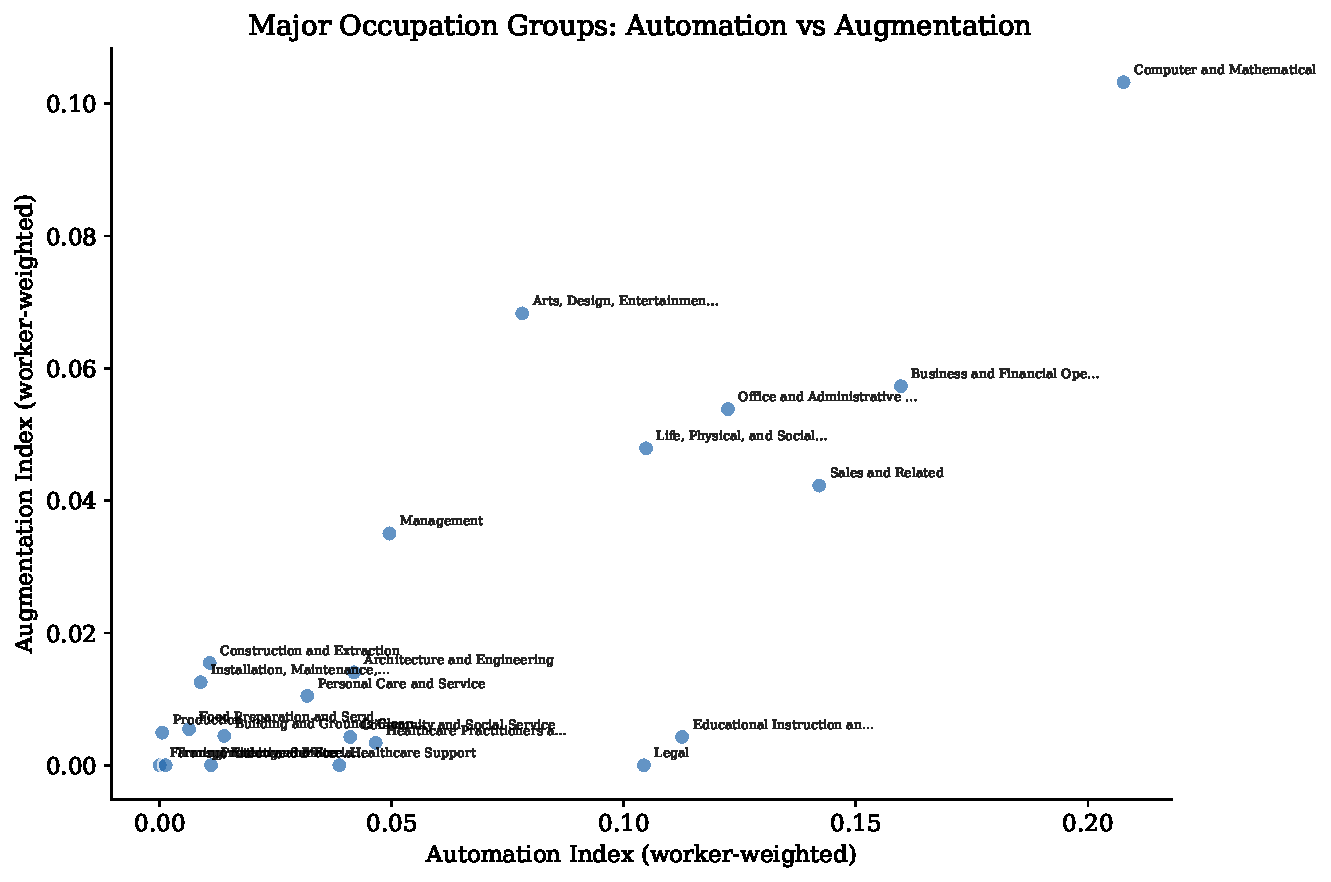
\includegraphics[width=0.85\textwidth]{auto_vs_aug_socgr.pdf}
\caption{Major occupation groups ($\sim$22 CPS categories), worker-weighted averages of the detailed-occupation indices.  All groups labeled.}
\label{fig:socgr}
\end{figure}

\begin{figure}[H]
\centering
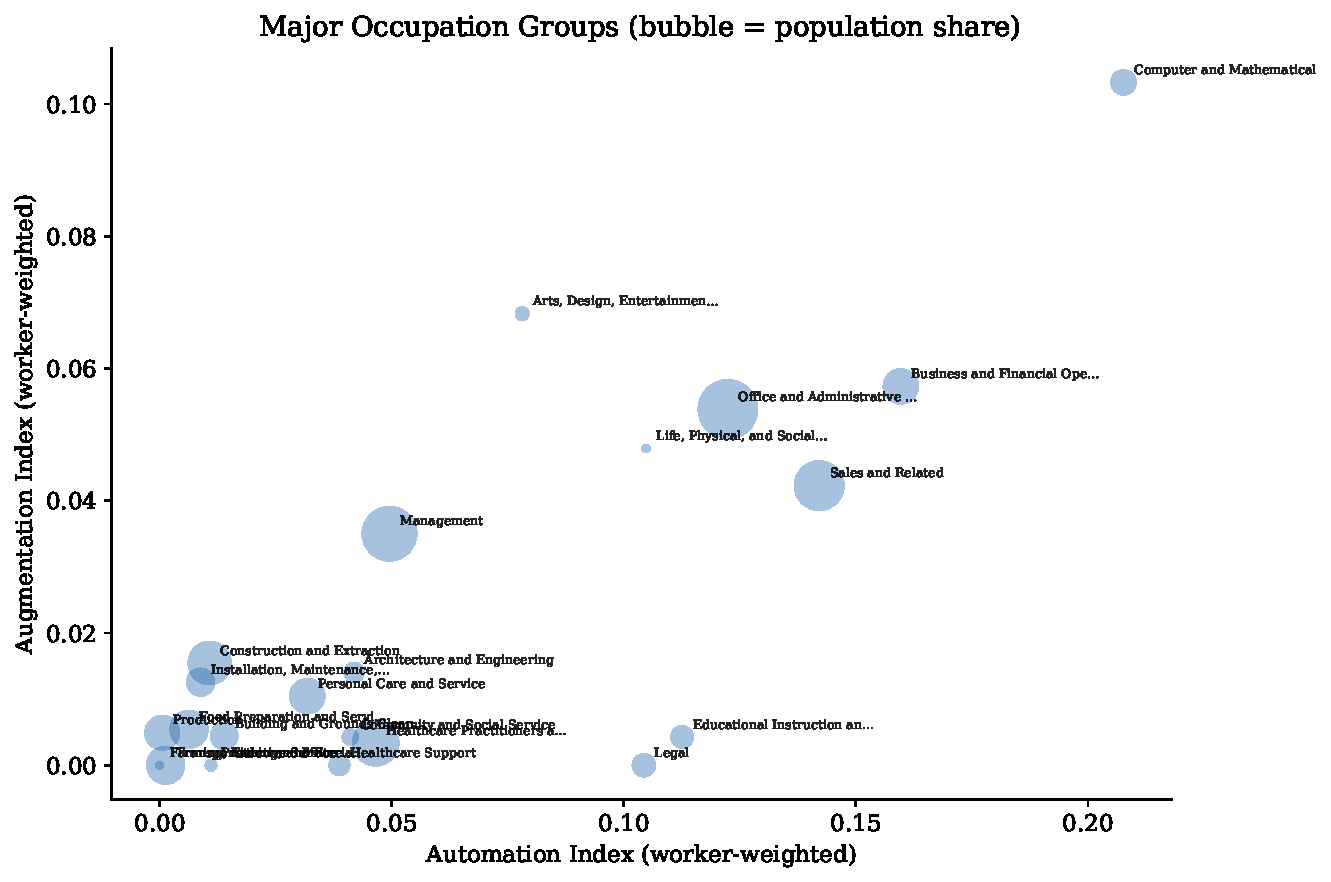
\includegraphics[width=0.85\textwidth]{auto_vs_aug_socgr_bubble.pdf}
\caption{Same as Figure~\ref{fig:socgr}, with bubble size proportional to the group's share of total CPS employment.}
\label{fig:socgr_bubble}
\end{figure}

%==================================================
\section{What This Enables}
%==================================================

\begin{enumerate}
  \item \textbf{Horse-race regressions}: with two independent indices, one can test whether automation or augmentation (or both) predicts labor market outcomes:
  \[
    Y_{it} = \alpha + \sum_{t} \beta_t (\mathbf{1}[t] \times \text{AutoIndex}_i) + \sum_{t} \gamma_t (\mathbf{1}[t] \times \text{AugIndex}_i) + \cdots
  \]
  If $\hat\beta_t > 0$ and $\hat\gamma_t \approx 0$ post-2022: automation drives displacement, augmentation does not.

  \item \textbf{Refinement of exposure measures}: existing measures (Eloundou, Felten, Webb) conflate substitution and complementarity.  The Bloom decomposition allows researchers to separate these channels without requiring proprietary interaction-type labels.

  \item \textbf{Connection to theory}: the automation index maps onto $s(i)$ in task-based models (the AI supply shock that displaces workers), while the augmentation index maps onto the augmentation channel that most models set aside as ``future work.''
\end{enumerate}

%==================================================
\section{Limitations and Next Steps}
%==================================================

\begin{itemize}
  \item The Bloom verb classification involves judgment calls (e.g.\ ``Apply'' as automation rather than augmentation).  Sensitivity checks moving level 3 to the augmentation side are needed.
  \item O*NET task verbs are standardized and may not capture the full nuance of how AI is used in practice.  The Anthropic penetration score mitigates this by weighting only tasks with revealed usage.
  \item The penetration data reflects Claude usage specifically, not all AI tools.  Generalizability to GPT-4, Gemini, or domain-specific AI is an open question.
  \item Empirical results (DiD regressions using these indices) are preliminary and not reported here.
\end{itemize}

\bigskip
\noindent\textbf{Next steps}: run the horse-race regressions on CPS-ASEC unemployment and wage outcomes; validate against Anthropic's aggregate 57/43 augmentation-automation split; explore whether the automation index predicts displacement more strongly than existing exposure measures.

\end{document}
